% Apresentações em widescreen. Outros valores possíveis: 1610, 149, 54, 43 e 32.
% Por padrão, as apresentações são no formato 4:3 (sem o aspectratio).
%\documentclass[aspectratio=169]{beamer}
\documentclass{beamer}

\usetheme[]{Madrid}
%\usetheme{Singapore}
\useoutertheme{miniframes}%\useoutertheme{infolines}
\usecolortheme{default}
\usefonttheme[onlymath]{serif}      % para fontes matemáticas
% Encontre mais temas e cores em http://www.hartwork.org/beamer-theme-matrix/ 
% Veja também http://deic.uab.es/~iblanes/beamer_gallery/index.html

%footline do infolines (Padrão do tema Madrid)
\setbeamertemplate{footline}
{%
   \leavevmode%
   \hbox{%
      \begin{beamercolorbox}[wd=.2\paperwidth,ht=2.25ex,dp=1ex,center]{author in head/foot}%
         \usebeamerfont{author in head/foot}\insertshortauthor
      \end{beamercolorbox}%
      \begin{beamercolorbox}[wd=.7\paperwidth,ht=2.25ex,dp=1ex,center]{title in head/foot}%
         \usebeamerfont{title in head/foot}\insertshorttitle
      \end{beamercolorbox}%
      \begin{beamercolorbox}[wd=.1\paperwidth,ht=2.25ex,dp=1ex,center]{date in head/foot}%
         \usebeamertemplate{page number in head/foot}\hspace*{2ex} 
      \end{beamercolorbox}
   }%
   \vskip0pt%
}
%footline do infolines (Pardrão do tema Singapore)
\setbeamertemplate{headline}
{%
   \begin{beamercolorbox}[colsep=1.5pt]{upper separation line head}
   \end{beamercolorbox}
   \begin{beamercolorbox}{section in head/foot}
      \vskip2pt\insertnavigation{\paperwidth}\vskip2pt
   \end{beamercolorbox}%
   \begin{beamercolorbox}[colsep=1.5pt]{lower separation line head}
   \end{beamercolorbox}
}

% Customizações de Cores: fg significa cor do texto e bg é cor do fundo
\setbeamercolor{normal text}{fg=black}
\setbeamercolor{alerted text}{fg=blue}
\setbeamercolor{author}{fg=black}
\setbeamercolor{institute}{fg=black}
\setbeamercolor{date}{fg=green}
\setbeamercolor{frametitle}{fg=white}
\setbeamercolor{framesubtitle}{fg=brown}
\setbeamercolor{block title}{bg=blue, fg=white}   %Cor do título
\setbeamercolor{block body}{bg=gray, fg=darkgray} %Cor do texto (bg= fundo; fg=texto)

% ---
% Fontes
% ---
% Usar font 'TeX Gyre Termes' como fonte principal
\usepackage{tgtermes}
\usepackage{fontawesome5}       % Permite o uso da fonte Font Awesome

\usepackage[T1]{fontenc}        % Compilar correctamente com pdflatex
\usepackage[utf8]{inputenc}     % Codificacao do documento (conversão automática dos acentos).
\usepackage{ucs}                % Complemento do anterior.

% ---
% PACOTES
% ---
\usepackage[brazil]{babel}    % Idioma do documento
\usepackage{color}      % Controle das cores
\usepackage{txfonts}      % Fontes virtuais

\usepackage{amsthm, thmtools}          % Para teoremas
\usepackage{amssymb}                   % Para exibir símbolos de conjuntos de números (reais, etc...).
\usepackage[mathscr]{eucal}            % Outras fontes (\mathscr)
\usepackage{amsmath}                   % Para adcionar equações
\usepackage{amsfonts}                  % Fontes para notação matemática. de cada seção.
\usepackage{esint}                     % Vários simbolos integrais
\usepackage{mathtools}                 %
\usepackage{xfrac}                     %

\usepackage{graphicx}                   % Insercao de figuras
\usepackage{wrapfig}                    % Insercao de figuras junto ao texto
\usepackage[caption = false]{subfig}    % Insercao de subfiguras
\usepackage{caption}                    % Insercao de legendas nas figuras
\usepackage{float}                      % Para posicionar figuras corretamente.

\usepackage{hyperref}


\usepackage{xcolor}  % see https://latexcolor.com/
\definecolor{codegreen}{rgb}{0,0.6,0}
\definecolor{codegray}{rgb}{0.5,0.5,0.5}
\definecolor{amaranth}{rgb}{0.9, 0.17, 0.31}
\definecolor{theBlack}{gray}{0.0}
\definecolor{theWhite}{gray}{0.9}

% ------------------------------------------------------------------------------
% PARA EXIBIÇÃO DE CÓDIGO FONTE
% ------------------------------------------------------------------------------
% see https://en.wikibooks.org/wiki/LaTeX/Source_Code_Listings
\usepackage{listings}
\lstset{
   backgroundcolor=\color{gray!5!white},   % choose the background color; you must add \usepackage{color} or \usepackage{xcolor}; should come as last argument
   basicstyle=\mdseries\ttfamily\tiny\color{black}, % the size of the fonts that are used for the code
   breakatwhitespace=false,         % sets if automatic breaks should only happen at whitespace
   breaklines=true,                 % sets automatic line breaking
   captionpos=t,                    % sets the caption-position to bottom
   columns=fixed,                   % Using fixed column width (for e.g. nice alignment)
   escapechar=µ,
   numbers=none,                    % Not use numbers
   keepspaces=true,                 % keeps spaces in text, useful for keeping indentation of code (possibly needs columns=flexible)
   showspaces=false,                % show spaces everywhere adding particular underscores; it overrides 'showstringspaces'
   showstringspaces=false,          % underline spaces within strings only
   showtabs=false,                  % show tabs within strings adding particular underscores
   tabsize=3, 	                     % sets default tabsize to 3 spaces
   %frame=single,	                  % adds a frame around the code
   %rulecolor=\color{black},         % if not set, the frame-color may be changed on line-breaks within not-black text (e.g. comments (green here))
}

\lstdefinestyle{c}{
   language=C, % the language of the code (can be overrided per snippet)
   commentstyle=\color{codegray}, % comment style
   keywordstyle={\color{codegreen}\bfseries},
   stringstyle=\color{amaranth} % string literal style
}

\lstdefinestyle{f90}{
   language=Fortran, % the language of the code (can be overrided per snippet)
   commentstyle=\color{codegray}, % comment style
   keywordstyle={\color{codegreen}\bfseries},
   stringstyle=\color{amaranth} % string literal style
}

\lstdefinestyle{py}{
   language=Python, % the language of the code (can be overrided per snippet)
   commentstyle=\color{codegray}, % comment style
   keywordstyle={\color{codegreen}\bfseries},
   stringstyle=\color{amaranth} % string literal style
}


% ---

% --- Informações do documento ---
\title{
  Solução numérica de sistemas dinâmicos
}
\author{I. F. F. dos{ }Santos}
\institute{
   Universidade Federal de Alagoas\\
   Instituto de Física
}
\date{}
% ---

% ----------------- INÍCIO DO DOCUMENTO --------------------------------------
\begin{document}

% ----------------- NOVO SLIDE --------------------------------
\begin{frame}

\begin{minipage}{1\linewidth}
   \centering
   \begin{tabular}{ccc}
      \begin{tabular}{c}
         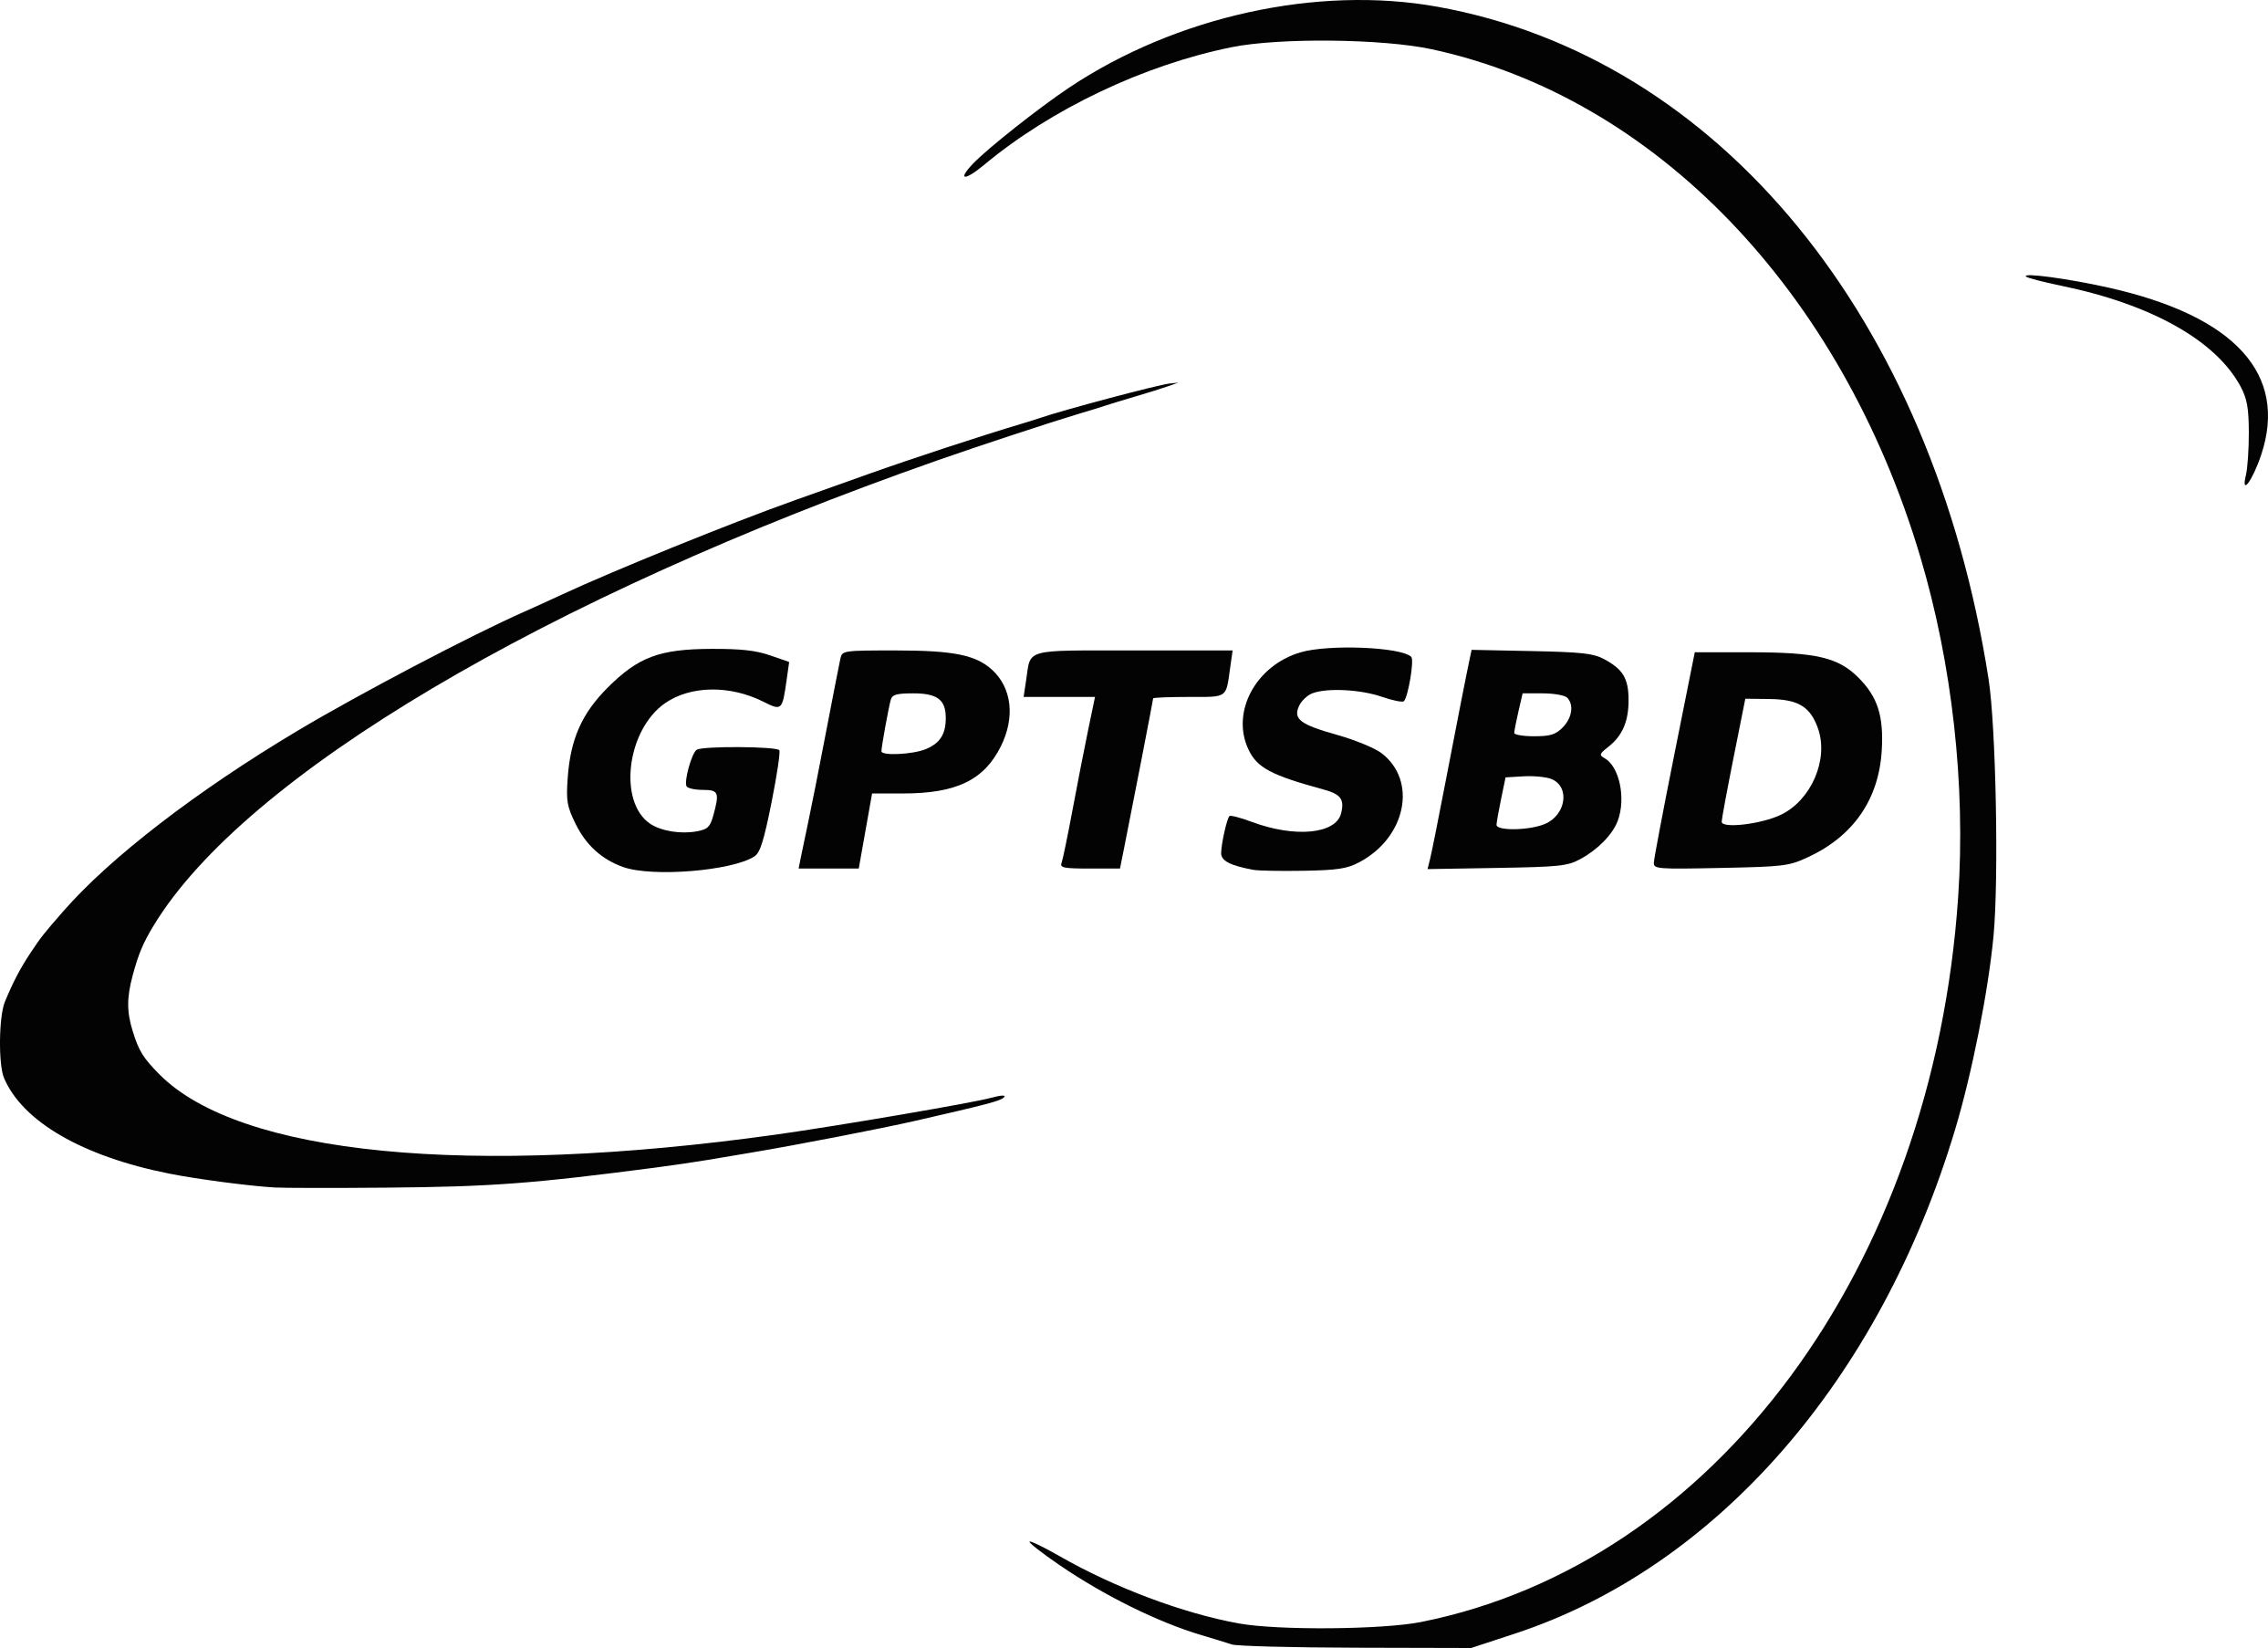
\includegraphics[width=2.5cm]{img/gptsdb}
      \end{tabular}
      &
      \begin{tabular}{c}
         
\includegraphics[width=1.0cm]{img/UFAL}
      \end{tabular}
      &
      \begin{tabular}{c}
         
\includegraphics[width=3.0cm]{img/IF}
      \end{tabular}
   \end{tabular}
\end{minipage}

\titlepage

\end{frame}

% ----------------- NOVO SLIDE --------------------------------
\begin{frame}{Sumário}
\tableofcontents
\end{frame}


\section{Introdução}

% ----------------- NOVO SLIDE --------------------------------
\begin{frame}{Sistemas dinâmicos}
   \begin{itemize}
      \item[{\color{black}$\mathcal E$}]
      Espaço d'estados:
      um conjunto onde cada ponto representa um possível estado
      do sistema físico,
      nesse caso um aberto de $\mathbb R^n$ ou $\mathbb C^n$.
      \item[{\color{black}$x(t)$}]
      Evolução:
      uma função do tempo
      que diz qual será o estado \textit{futuro}, após a evolução no tempo.
   \end{itemize}


   \begin{tabular}{cr}

      \begin{tabular}{c}\parbox{0.4\linewidth}{
         Em geral, uma lei de evolução é da forma
         \begin{equation}\label{eq:PVI}
            \frac{d}{dt} x(t) = F(t, x(t)),
         \end{equation}
         sujeito à condição de que $x(t_0) = x_0$.
      }\end{tabular} &

      \begin{tabular}{c}
         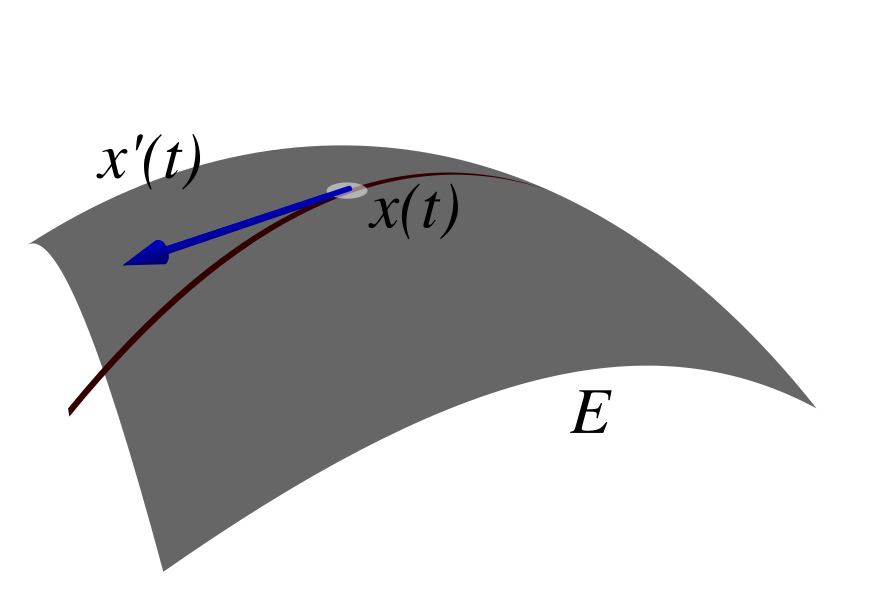
\includegraphics[width=0.4\textwidth]{img/Tangentialvektor}
      \end{tabular}
   \end{tabular}
\end{frame}

% ----------------- NOVO SLIDE --------------------------------
\begin{frame}{Problema de valor inicial}

   Problema: Dada uma função
   $F:\mathbb R\times\mathcal E\rightarrow\mathcal E$ e
   um estado inicial $x_0\in\mathcal E$
   no instante inicial $t_0\in\mathbb R$
   encontre uma evolução $x:\mathbb R\rightarrow\mathcal E$
   tal que a eq. \ref{eq:PVI} é satisfeita e $x(t_0) = x_0$.

   \vfill

   O PVI pode ser reescrito na sua forma integral usando o TFC
   \begin{equation}
      x(t_0 + \delta t) = x(t_0) +
      \int_{t_0}^{t_0 + \delta t} F(t, x(t)) ~ dt.
   \end{equation}

   \vfill

   \begin{itemize}
      \item Se $F$ é contínua então o PVI possui solução.
      \item Se $F$ é Lipschitz contínua no segundo argumento
      então o PVI possui uma única solução.
   \end{itemize}
\end{frame}

% ----------------- NOVO SLIDE --------------------------------
\begin{frame}[fragile]{Representando em \texttt C}
   No $\mathbb R^n$ ou $\mathbb C^n$,
   \[
      \begin{bmatrix}
         x_1(t_0 + \delta t) \\ \vdots \\ x_n(t_0 + \delta t)
      \end{bmatrix} =
      \begin{bmatrix} x_1(t_0) \\ \vdots \\ x_n(t_0) \end{bmatrix} +
      \int_{t_0}^{t_0 + \delta t}
      \begin{bmatrix}
         f_1(t, x(t)) \\ \vdots \\ f_n(t, x(t))
      \end{bmatrix} ~ dt
   \]

   \rule{\textwidth}{1pt}
   \scriptsize
\begin{lstlisting}[style = c]
typedef struct estado_s {
    // _Complex
   double *x;
   int dim;
} estado_t;

static inline double dot_x(int i, double t, estado_t sistema){ /* ... */ }

/* Inicialize da seguinte maneira */
estado_t sistema;
sistema.dim = /* ... */ ;
sistema.x = (double*)malloc((size_t)(sistema.dim) * sizeof(double));
\end{lstlisting}
   \rule{\textwidth}{1pt}

\end{frame}

% ----------------- NOVO SLIDE --------------------------------
\begin{frame}{Dicas}
   \begin{itemize}
      \item Simplifique seu problema, i.e.,
      resolva outro equivalente porém mais simples.
      \item Sempre que possível use variáveis adimensionais
      (defina $u = v_0^{-1} v$).
      \item Escalas quânticas ou astronômicas DEVEM ser reescaladas.
      \item Identifique os pontos fixos
      ($x^*\in\mathcal E$ t.q. $F(t, x^*) = 0$)
      e outros casos de solução conhecida.
      \item Identifique constantes de evolução,
      funções $f:\mathcal E\rightarrow\mathbb R$ tais que
      $f(x(t_0 + \delta t)) = f(x_0)$,
      e as use para testar sua solução.
   \end{itemize}
\end{frame}

\section{Problemas muito simples}

% ----------------- NOVO SLIDE --------------------------------
\begin{frame}[fragile]{Método de Euler}

   Método:
   \begin{equation}
      x(t_0 + \delta t) \leftarrow x_0 + F(t_0, x_0) ~ \delta t
   \end{equation}

   Recursão:
   \begin{align}
      x_0 &\leftarrow x(t_0 + \delta t) \\
      t_0 &\leftarrow t_0 + \delta t
   \end{align}

   \rule{\textwidth}{1pt}
   \scriptsize
\begin{lstlisting}[style = c]
t = t0;
while(t <= tf){
   for(int i = 0; i < sistema.dim; ++i) k[i] = dot_x(i, t, sistema);
   for(int i = 0; i < sistema.dim; ++i) sistema.x[i] += k[i] * dt;
   t += dt;
}
\end{lstlisting}
   \rule{\textwidth}{1pt}
\end{frame}

\subsection*{}

% ----------------- NOVO SLIDE --------------------------------
\begin{frame}[fragile]{Modelo SIR}

   \begin{itemize}
      \item $\mathcal E \sim \mathbb R^3$.
      \item Lei de evolução:
      \begin{equation}
         \frac{d}{dt}
         \begin{bmatrix} S \\ I \\ R \end{bmatrix} =
         \begin{bmatrix}
            -\frac{\beta}{N} S I \\
            \frac{\beta}{N} S I - \gamma I \\
            \gamma I
         \end{bmatrix}
         \quad\sim\quad
         \frac{d}{d\tau}
         \begin{bmatrix} s \\ i \\ r \end{bmatrix} =
         \begin{bmatrix}
            -\alpha ~ s i \\
            \alpha ~ s i - i \\
            i
         \end{bmatrix}
      \end{equation}
      onde $\alpha = \sfrac{\beta}{\gamma}$,
      $\tau = \gamma t$,
      $s = \frac{1}{N} S$,
      $i = \frac{1}{N} I$ e
      $r = \frac{1}{N} R$.
      \item $N = S + I + R$ é uma constante de evolução.
   \end{itemize}

   \rule{\textwidth}{1pt}
   \scriptsize
\begin{lstlisting}[style = c]
typedef struct estado_s { double S, I, R; } estado_t;

static inline double dot_S(estado_t sistema){
   return (alpha * sistema.S * sistema.I);
}

static inline double dot_R(estado_t sistema){
   return (sistema.I);
}
static inline double N(estado_t sistema){
   return (sistema.S + sistema.I + sistema.R);
}
\end{lstlisting}

\end{frame}

% ----------------- NOVO SLIDE --------------------------------
\begin{frame}[fragile]{Modelo SIR}%
   \begin{center}
      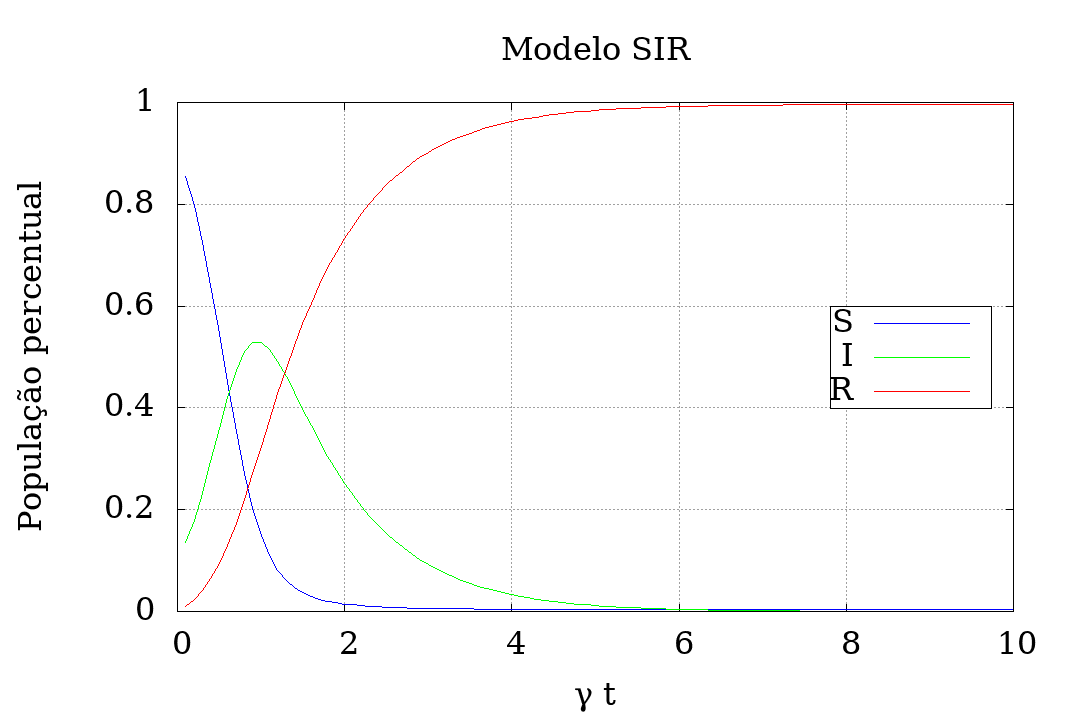
\includegraphics[width=0.5\textwidth]{code/SIR.png}
   \end{center}

\scriptsize
\begin{lstlisting}[style = c]
t = 0.0;
while(t <= tf){
   k_S = dot_S(sistema) * dt;
   k_I = dot_R(sistema) * dt;
   sistema.S -= k_S;
   sistema.I += k_S - k_I;
   sistema.R += k_I;
   t += dt;
   if(fabs(N(sistema) - 1.0) > 1.0e-8)
      fputs("A populacao nao estah conservando.\n", stderr);
}
\end{lstlisting}

\end{frame}

\section{Sistemas hamiltonianos}

% ----------------- NOVO SLIDE --------------------------------
\begin{frame}[fragile]{Equações de Hamilton}
   \begin{itemize}
      \item $\mathcal E \sim \mathbb R^{2f}$,
      $\mathcal H:\mathcal E\rightarrow\mathbb R$.
      \item Leis de evolução:
      \begin{equation}
         \frac{d}{dt}
         \begin{bmatrix} q(t) \\ p(t) \end{bmatrix} =
         \begin{bmatrix} v(t, q(t), p(t)) \\ f(t, q(t), p(t)) \end{bmatrix} =
         \begin{bmatrix}
            \frac{\partial}{\partial p}\mathcal H\\
            -\frac{\partial}{\partial q}\mathcal H
         \end{bmatrix}
      \end{equation}
      \item $E = \mathcal H$ é uma constante de evolução.
   \end{itemize}


   \rule{\textwidth}{1pt}
   \scriptsize
\begin{lstlisting}[style = c]
typedef struct estado_s {
   double *Q, *P;
   int dim;
} estado_t;

static inline double dot_Q(int i, estado_t sistema){ /* ... */ }
static inline double dot_P(int i, estado_t sistema){ /* ... */ }
\end{lstlisting}
\end{frame}

% ----------------- NOVO SLIDE --------------------------------
\begin{frame}[fragile]{Método de Euler semi-implícito}

   {\scriptsize Derivada da forma $(v, f) = (v(t, q, p), ~ f(t, q))$.}

   Método:
   \begin{align}
      p(t_0 + \delta t) &\leftarrow p_0 + f(t_0, q_0) ~ \delta t \\
      q(t_0 + \delta t) &\leftarrow q_0 + v(t_0, q_0, p(t_0 + \delta t)) ~ \delta t
   \end{align}

   \rule{\textwidth}{1pt}
   \scriptsize
\begin{lstlisting}[style = c]
for(int i = 0; i < sistema.dim; ++i) k_P[i] = dot_P(i, sistema);
for(int i = 0; i < sistema.dim; ++i) sistema.P[i] += k_P[i] * dt;
for(int i = 0; i < sistema.dim; ++i) k_Q[i] = dot_Q(i, sistema);
for(int i = 0; i < sistema.dim; ++i) sistema.Q[i] += k_Q[i] * dt;
\end{lstlisting}
   \rule{\textwidth}{1pt}
\end{frame}

% ----------------- NOVO SLIDE --------------------------------
\begin{frame}[fragile]{Método de Verlet}

   {\scriptsize Derivada da forma $(\dot q, \dot p) = (v(t, p), ~ f(t, q, p))$.}

   Método:
   \begin{align}
      q(t_0 + {\textstyle\frac{1}{2}} \delta t) &\leftarrow q_0 + v(t_0, p_0) ~ {\textstyle\frac{1}{2}} \delta t \\
      p(t_0 + \delta t) &\leftarrow p_0 + f(t_0, q(t_0 + {\textstyle\frac{1}{2}} \delta t), p_0) ~ \delta t \\
      q(t_0 + \delta t) &\leftarrow q(t_0 + {\textstyle\frac{1}{2}} \delta t) + v(t_0, p(t_0 + \delta t)) ~ {\textstyle\frac{1}{2}} \delta t
   \end{align}

   \rule{\textwidth}{1pt}
   \scriptsize
\begin{lstlisting}[style = c]
dt2 = 0.5 * dt;
for(int i = 0; i < sistema.dim; ++i) k_Q[i] = dot_Q(i, sistema);
for(int i = 0; i < sistema.dim; ++i) sistema.Q[i] += k_Q[i] * dt2;
for(int i = 0; i < sistema.dim; ++i) k_P[i] = dot_P(i, sistema);
for(int i = 0; i < sistema.dim; ++i) sistema.P[i] += k_P[i] * dt;
for(int i = 0; i < sistema.dim; ++i) k_Q[i] = dot_Q(i, sistema);
for(int i = 0; i < sistema.dim; ++i) sistema.Q[i] += k_Q[i] * dt2;
\end{lstlisting}
   \rule{\textwidth}{1pt}
\end{frame}

% ----------------- NOVO SLIDE --------------------------------
\begin{frame}[fragile]{Método de Verlet}

   \rule{\textwidth}{1pt}
   \scriptsize
\begin{lstlisting}[style = c]
/* OU ainda */
for(int i = 0; i < sistema.dim; ++i){
   k_Q[i] = dot_Q(i, sistema);
   sistema.Q[i] += k_Q[i] * dt2;
}
for(int i = 0; i < sistema.dim; ++i) k_P[i] = dot_P(i, sistema);
for(int i = 0; i < sistema.dim; ++i) sistema.P[i] += k_P[i] * dt;
for(int i = 0; i < sistema.dim; ++i){
   k_Q[i] = dot_Q(i, sistema);
   sistema.Q[i] += k_Q[i] * dt2;
}
\end{lstlisting}
   \rule{\textwidth}{1pt}
\end{frame}

\subsection*{}

% ----------------- NOVO SLIDE --------------------------------
\begin{frame}[fragile]{Oscilador vertical}

   \begin{itemize}
      \item $\mathcal E \sim \mathbb R^2$.
      \item Lei de evolução:
      \begin{equation}
         \frac{d}{dt}
         \begin{bmatrix} y \\ p \end{bmatrix} =
         \begin{bmatrix}
            \frac{1}{m} p \\
            -k y - \frac{\beta}{m} p  - m g
         \end{bmatrix}
         \quad\sim\quad
         \frac{d}{d\tau}
         \begin{bmatrix} Q \\ P \end{bmatrix} =
         \begin{bmatrix} P \\ -(Q + \gamma P) + 1 \end{bmatrix}
      \end{equation}
      onde $\gamma = \frac{\beta}{m}\sqrt{\frac{m}{k}}$,
      $\tau = \sqrt{\frac{k}{m}} t$,
      $Q = - \frac{k}{mg} y$ e
      $P = - \frac{1}{mg} \sqrt{\frac{k}{m}} p$.
   \end{itemize}

   \rule{\textwidth}{1pt}
   \scriptsize
\begin{lstlisting}[style = c]
typedef struct estado_s { double Q, P; } estado_t ;
static inline double dot_Q(estado_t sistema){
   return (sistema.P);
}
static inline double dot_P(estado_t sistema){
   return (-(sistema.Q + gamma * sistema.P) + 1.0);
}
\end{lstlisting}
\end{frame}

% ----------------- NOVO SLIDE --------------------------------
\begin{frame}[fragile]{Oscilador vertical}%
   \begin{center}
      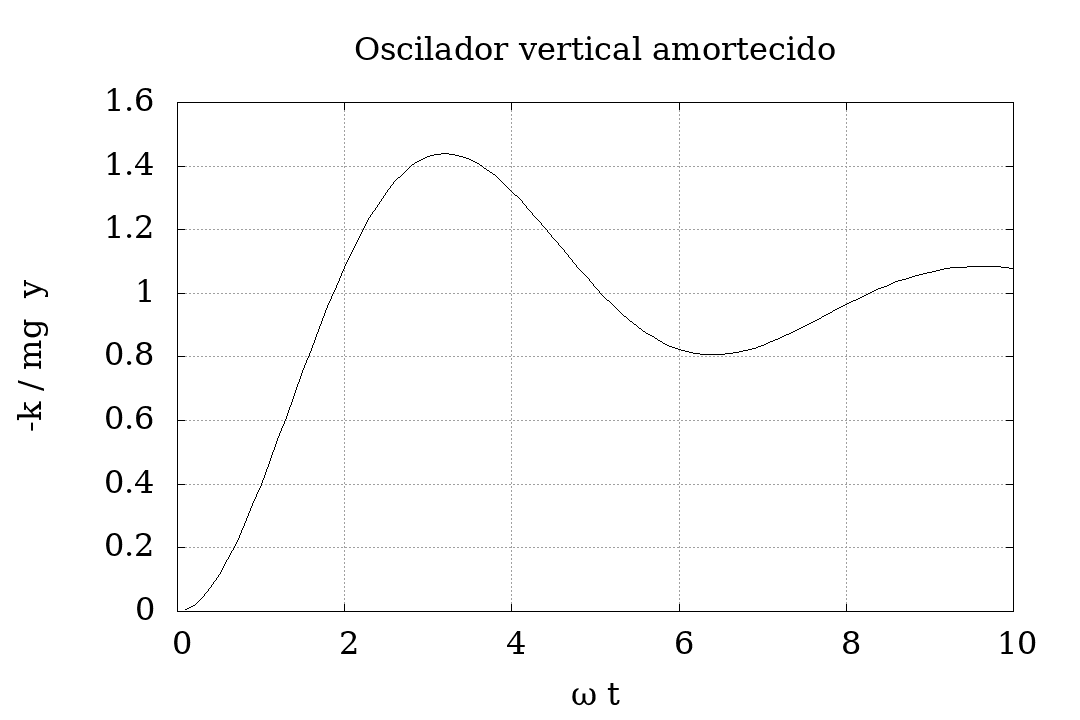
\includegraphics[width=0.4\textwidth]{code/oscilador.png}
      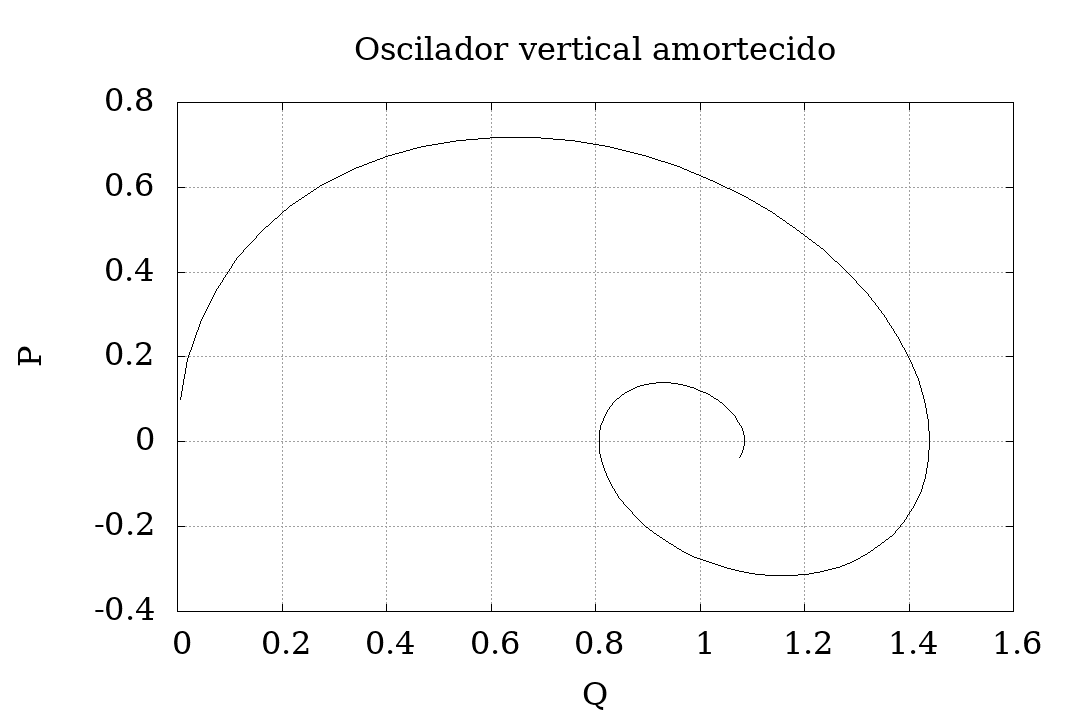
\includegraphics[width=0.4\textwidth]{code/oscilador_PS.png}
   \end{center}
   \rule{\textwidth}{1pt}
   \scriptsize
\begin{lstlisting}[style = c]
/* Com Euler */
sistema.Q += dot_Q(sistema) * dt;
sistema.P += dot_P(sistema) * dt;

/* Com Verlet */
dt2 = 0.5 * dt;
sistema.Q += dot_Q(sistema) * dt2;
sistema.P += dot_P(sistema) * dt;
sistema.Q += dot_Q(sistema) * dt2;
\end{lstlisting}
   \rule{\textwidth}{1pt}
\end{frame}

% ----------------- NOVO SLIDE --------------------------------
\begin{frame}[fragile]{Cadeia de massas idênticas com interação linear}

   \begin{itemize}
      \item $\mathcal E \sim \mathbb R^{2N}$.
      \item Lei de evolução:
      \begin{equation}
         \frac{d}{dt}
         \begin{bmatrix} q_n \\ p_n \end{bmatrix} =
         \begin{bmatrix}
            \frac{1}{m} p_n \\
            k (q_{n-1} + 2 q_n + q_{n+1})
         \end{bmatrix}
         \quad\sim\quad
         \frac{d}{d\tau}
         \begin{bmatrix} Q_n \\ P_n \end{bmatrix} =
         \begin{bmatrix} P_n \\ Q_{n-1} + 2 Q_n + Q_{n+1} \end{bmatrix}
      \end{equation}
      onde
      $\tau = \sqrt{\frac{k}{m}} t$,
      $Q_n = q_0^{-1} q_n$ e
      $P_n = q_0 \sqrt{m k} ~ p_n$.
   \end{itemize}

   \rule{\textwidth}{1pt}
   \scriptsize
\begin{lstlisting}[style = c]
typedef struct estado_s { double Q, P; int N; } estado_t ;
static inline double dot_Q(int n, estado_t *sistema){
   return (sistema.P[n]);
}
static inline double dot_P(int n, estado_t sistema){
   return (sistema.Q[n-1] - 2.0 * sistema.Q[n] + sistema.Q[n+1]);
}
\end{lstlisting}
   \rule{\textwidth}{1pt}
\end{frame}

% ----------------- NOVO SLIDE --------------------------------
\begin{frame}[fragile]{Cadeia de massas idênticas com interação linear}
   \rule{\textwidth}{1pt}
   \scriptsize
\begin{lstlisting}[style = c]
/* Com Verlet */
for(int n = 1; n <= sistema.dim; ++n){
   k_Q[n] = dot_Q(n, sistema);
   sistema.Q[n] += k_Q[n] * dt2;
}
for(int n = 1; n <= sistema.dim; ++n){
   k_P[n] = dot_P(n, sistema);
   sistema.P[n] += k_P[n] * dt;
}
for(int n = 1; n <= sistema.dim; ++n){
   k_Q[n] = dot_Q(n, sistema);
   sistema.Q[n] += k_Q[n] * dt2;
}
\end{lstlisting}
   \rule{\textwidth}{1pt}
\end{frame}

\section{Problemas genéricos}

% ----------------- NOVO SLIDE --------------------------------
\begin{frame}[fragile]{Mudança de variáveis}
   \begin{itemize}
      \item $s:\mathbb R\rightarrow\mathbb R:t\mapsto \tau$
      \item $T:\mathcal E\rightarrow\mathcal E:x\mapsto y$
      \item $y(\tau) = Tx(s^{-1}(\tau))$
      \item $G(\tau, y(\tau)) =
      \frac{d}{d\tau} s^{-1}(\tau) ~ T F(s^{-1}(\tau), T^{-1}(y(\tau)))$
   \end{itemize}

   \begin{equation}
      \frac{d}{dt} x(t) = F(t, x(t))
      \quad\sim\quad
      \frac{d}{d\tau} y(\tau) = G(\tau, y(\tau))
   \end{equation}
\end{frame}

% ----------------- NOVO SLIDE --------------------------------
\begin{frame}{Outros métodos}
   \begin{itemize}
      \item \href{https://pt.wikipedia.org/wiki/Lista_de_m\%C3\%A9todos_Runge-Kutta}{Runge-Kutta}
      \item \href{https://pt.wikipedia.org/wiki/M\%C3\%A9todo_de_passo_m\%C3\%BAltiplo}{Adams}
      \item \href{https://pt.wikipedia.org/wiki/Integrador_simpl\%C3\%A9tico}{Integradores simpléticos}
   \end{itemize}
\end{frame}

% ----------------- FIM DO DOCUMENTO -----------------------------------------
\end{document}
